\documentclass[12pt]{beamer}
\usetheme{CambridgeUS}
\usecolortheme{dolphin}
\usepackage[utf8]{inputenc}
\usepackage{amsmath}
\usepackage{amsfonts}
\usepackage{amssymb}
\usepackage{graphicx}
\usepackage{mathtools}
\usepackage{multimedia}
\usepackage[mathscr]{euscript}
\usepackage{xcolor}
\usepackage{algorithmicx}
\usepackage{algpseudocode}
\usepackage{setspace}
\usepackage{listings}
\usepackage{xcolor}
\usepackage{textcomp}
\usepackage{subfigure}
\usepackage[overlay,absolute]{textpos}


\usepackage{color}
\definecolor{hellgelb}{rgb}{1,1,0.97}
\definecolor{colKeys}{rgb}{0,0,1}
\definecolor{colIdentifier}{rgb}{0,0,0}
\definecolor{colComments}{rgb}{0,.5,0}
\definecolor{colString}{rgb}{0,0.5,0}
\lstset{
	language=Matlab,
	float=hbp,
	basicstyle=\footnotesize\ttfamily,
	identifierstyle=\color{colIdentifier},
	keywordstyle=\color{colKeys},
	stringstyle=\color{colString},
	commentstyle=\itshape\color{colComments},
	columns=fixed,
	tabsize=4,
	frame=single,
	framerule=1pt,
	extendedchars=true,
	showspaces=false,%
	showstringspaces=false,
	numbers=left,
	numberstyle=\tiny\ttfamily,
	numbersep=1em,
	breaklines=true,
	breakindent=10pt,
	backgroundcolor=\color{hellgelb},
	breakautoindent=true,
	captionpos=t,
	xleftmargin=1em,
	xrightmargin=\fboxsep
}

\DeclarePairedDelimiter{\abs}{\lvert}{\rvert}
\DeclarePairedDelimiter{\norm}{\lVert}{\rVert}

\newcommand{\R}{\mathbb{R}}
\newcommand{\C}{\mathbb{C}}
\newcommand{\Tau}{\mathcal{T}}
\newcommand{\AMz}{\underset{z}{arg\, min}}
\newcommand{\prox}{\text{prox}}

\newcommand{\worm}{WWWWWoooooooRRRRRmmmmmm}

\author[Mueller]{Kevin Mueller}
\title[Convex Clustering Intro]{Intro to Convex Clustering with Robust Extensions \\ \normalsize AMATH Masters Final Project}
\setbeamercovered{transparent} 
%\institute{University of Washington} 
\date{March 12 2016} 
\subject{Amath 575} 

\iffalse
To do:
-Should we call it an objective or loss function?  Need to be consistent.
-Add in plot comparing methods
-Image assumptions and regularizers slide needs to be finished
-How do we compute prox_{\| W \cdot \|_1} ? Should add in on L1 wavelet reg slide
-Finish conclusions
-Add in sources and citations throughout presentation
\fi

\begin{document}

% Title Page
\begin{frame}
\titlepage
\end{frame}

% Contents
\begin{frame}{Contents}
\tableofcontents
\end{frame}

% MOTIVATION
\section{Motivation}


% Why Clustering?
\begin{frame}{Why Clustering?}
\begin{itemize}
	\item It is an unsupervised technique, which means that it does not require labeled data.
	\item Broad set of techniques for identifying subgroups in a data set. 
		\begin{itemize}
			\item K-Means \\
			\item Gaussian Mixture Models (Expectation Maximization) \\
			\item Spectral Clustering
			\item Hierarchal Clustering
			\item Convex Clustering
		\end{itemize}
\end{itemize}
\end{frame}

\section{K-Means}
% Problem Formulation
% OBJECTIVE FUNCTIONS
\begin{frame}{K-Means Formulation}
\begin{itemize}
	\item Given Data Points $\{ x_j \}_{j=1}^N$\\
	\item We seek to find a set of $k$ subgroups (index sets) $\{S_i \}_{i=1}^k$
	\item Let $\{\theta_i\}_{i=1}^k$ be the cluster centers
\end{itemize}
$$ \min_S \sum_{i=1}^k \sum_{j \in S_i} \lVert x_j - \theta_i \rVert^2 $$
$$ \text{s.t} \quad \theta_i = \frac{1}{\text{card } S_i} \sum_{j \in S_i} x_j $$
$$ \bigcup_{i=1}^k S_i = \left\{1,\dots,N\right\} $$
\end{frame}



% Kmeans formulation
\begin{frame}
	\begin{center}
		\vspace{3 mm}
		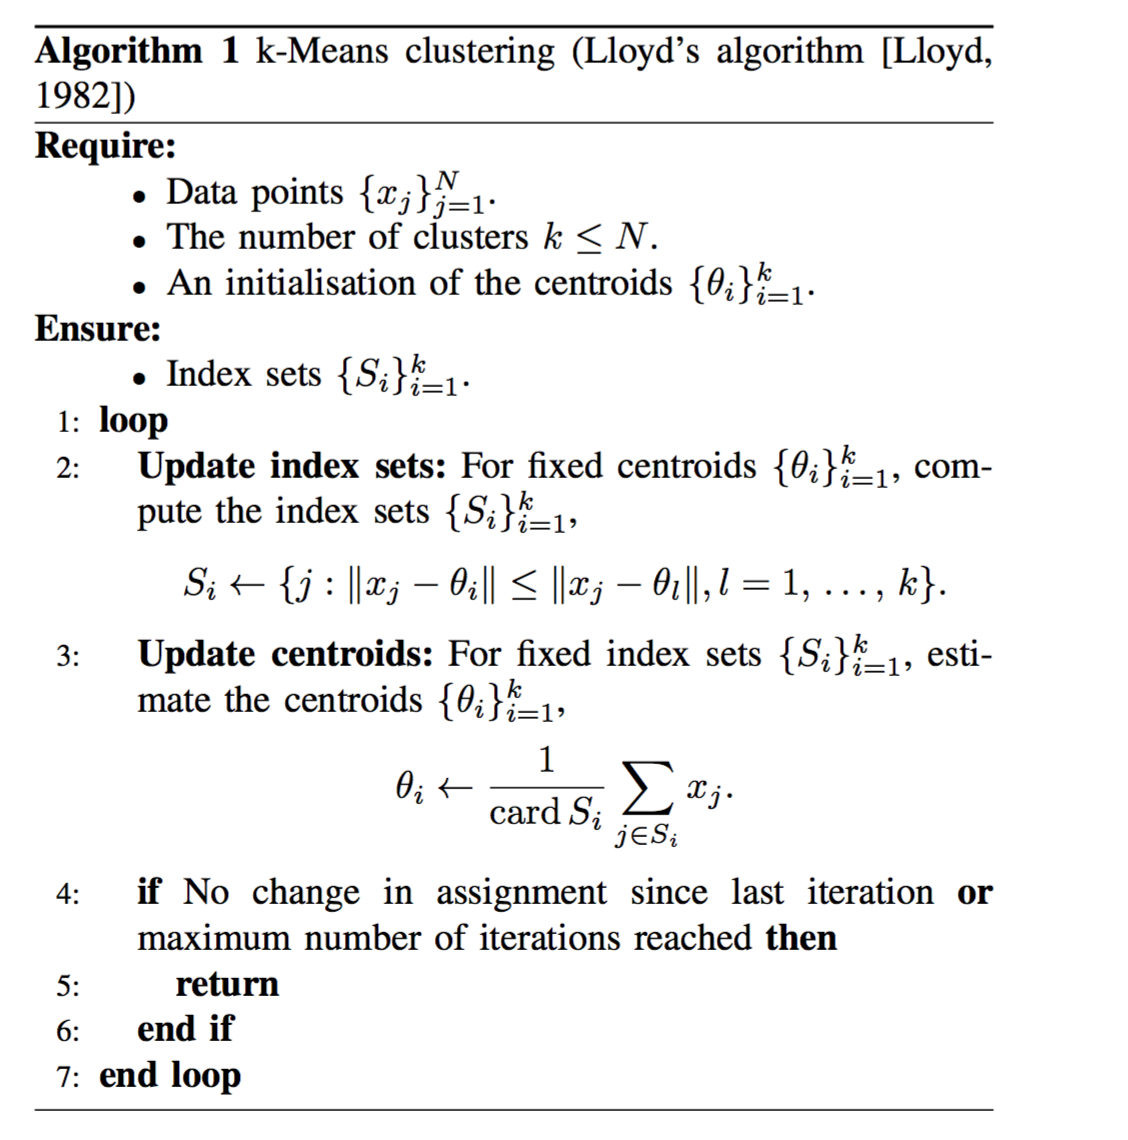
\includegraphics[scale=0.40]{../figures/Kmeans_Algorithm.png}
	\end{center}
\end{frame}

% Kmeans pictoral explanation
\begin{frame}
	\begin{center}
		\vspace{-3 mm}
		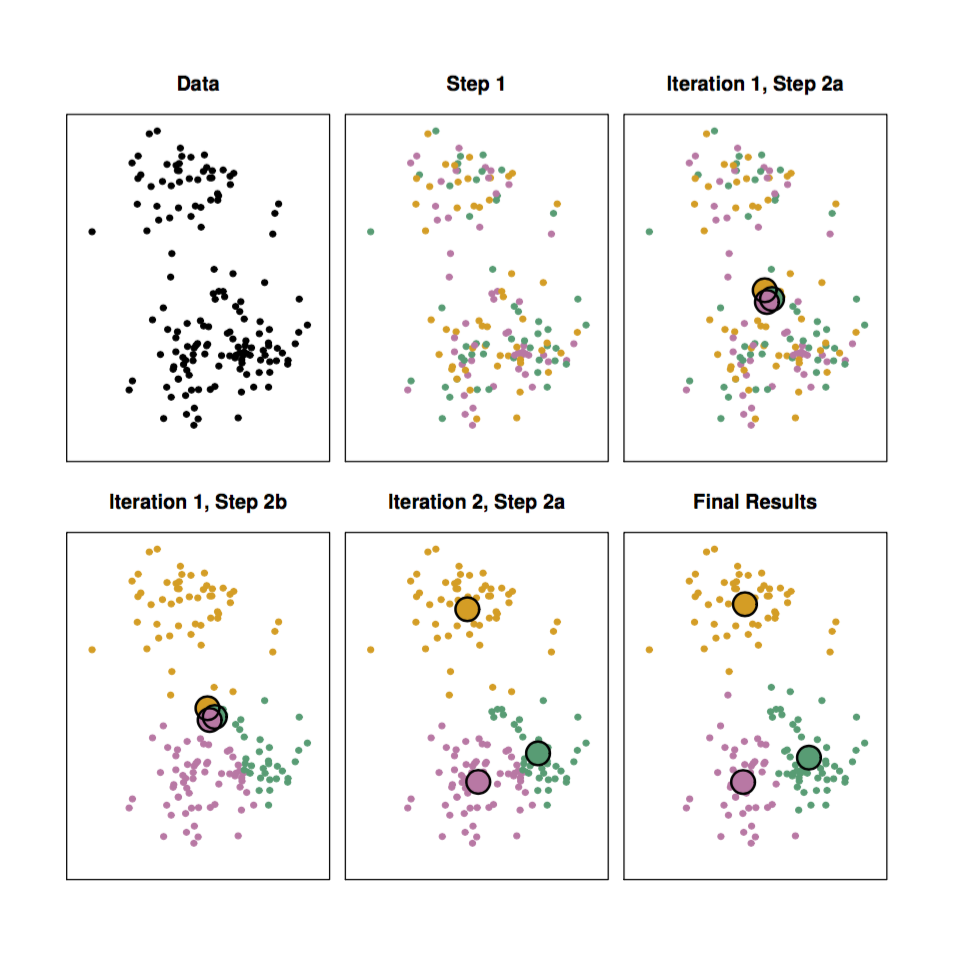
\includegraphics[scale=0.5]{../figures/Kmeans_example.png}
	\end{center}
\end{frame}

% Problems with Kmeans
\begin{frame}{Problems with K-Means}
	\begin{itemize}
		\item Requires an initialization of $k$ clusters
		\item Can yield different clusters for different initial conditions 
	\end{itemize}
	\begin{center}
		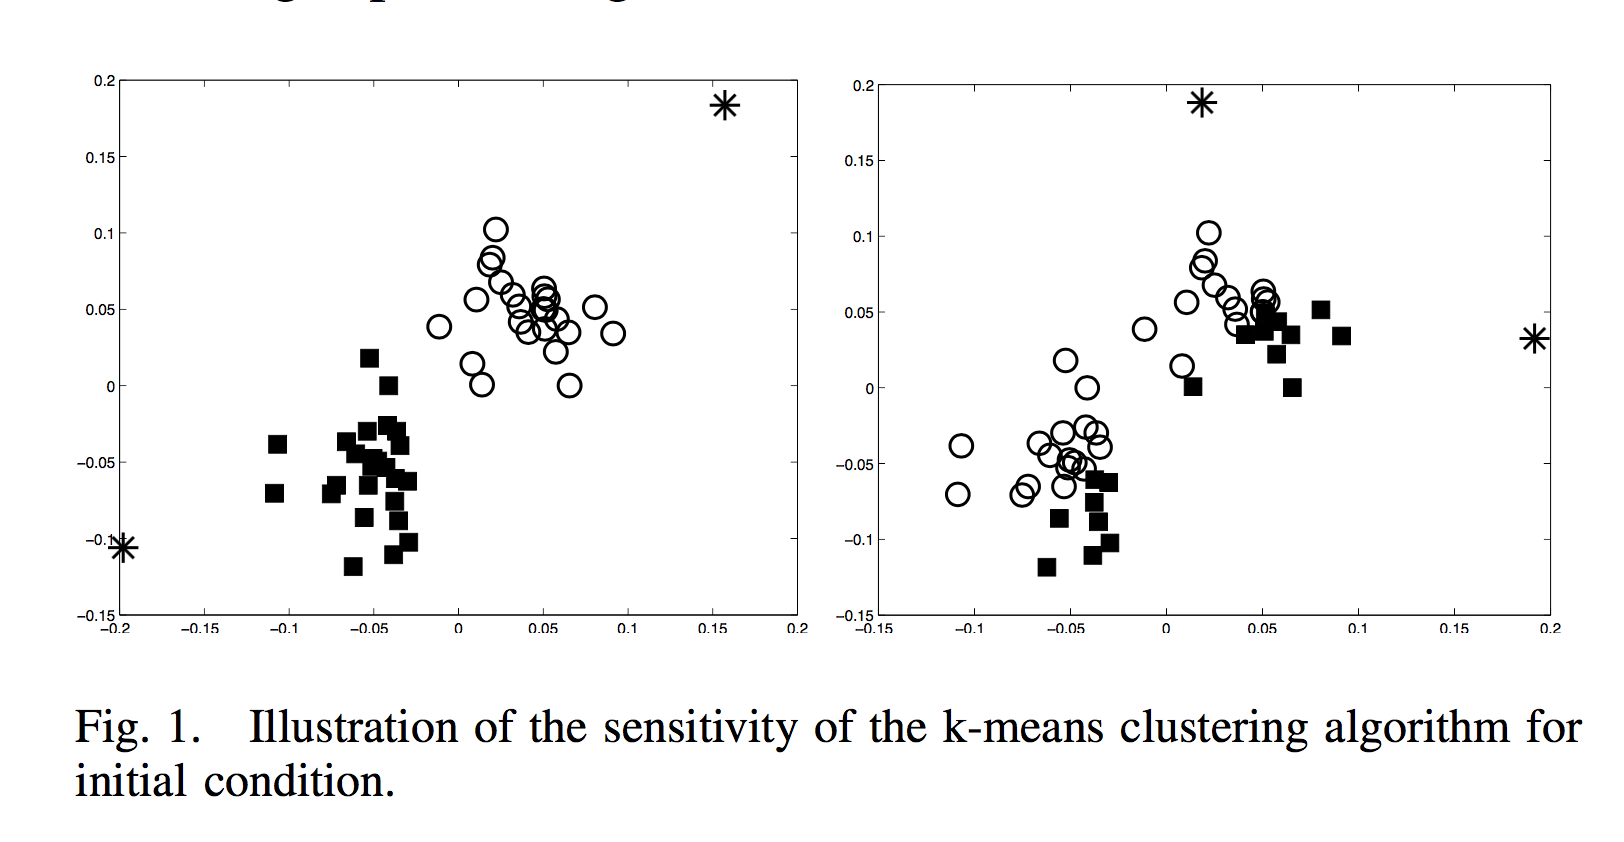
\includegraphics[scale=0.3]{../figures/Kmeans_diffclusters.png}
	\end{center}	

\end{frame}

\begin{frame}{Convex Relaxation}
	If we suppose there is a unique optima for the k-means formulation $S^*$, which is a partitioning of the set $\{1,\dots,N\}$ into k non-empty disjoint subsets. Then we can rewrite the k-means objective as,
	
	$$
	\begin{aligned}
	&\min_\mu \sum_{j=1}^N \lVert x_j - \mu_j \rVert^2 \\
	&\text{s.t} \{\mu_1,\dots,\mu_n\} \space \text{ contains k unique vectors}
	\end{aligned}
	$$
	
	Where $\mu \in \mathbb{R}^d$ for $j=1,\dots,N$ represents the cluster center for each point $x_j$. This would still give $k$ clusters assuming that $x$'s belong to the same cluster if their corresponding centroids are the same.
\end{frame}

% Convex Formulation
\section{Convex Formulation}

\begin{frame}{Convex Relaxation}
	We can reformulate the constraint by counting the unique vectors in the set $\{\mu_1,\dots,\mu_N \}$.
	Define an $\mathbb{R} \in N^2$ matrix as, $\Delta_{ij} = \kappa_(\mu_i,\mu_j)$ where $\kappa \space : \space \mathbb{R}^d \times \mathbb{R}^d \rightarrow \mathbb{R}$ has the symmetric property,
	$$ \kappa(\mu_i,\,\mu_j) = 0 \iff \mu_i = \mu_j$$
	
	An easy example of a $\kappa$ with these properties are the well known difference norms. In these case
	
	$$ \Delta =\left(\begin{array}{*{20}{c}}
0& \times & \cdots & \times \\
{}& \ddots & \ddots & \vdots \\
{}&{}& \ddots & \times \\
{}&{}&{}&0
\end{array}
\right)
$$
\end{frame}




\begin{frame}{Convex Relaxation}
	The number of vectors in the set $\{\mu_j \}_{j=n+1}^N$ that are equal to $\mu_n$, is the number of the zeros in the $n$th row of the upper upper triangle. Therefore to count the number of duplicates we can,
	
	\begin{itemize}
		\item Count the number of zeros in the first row of the upper triangle
		\item Count the number of zeros in the second row, unless there is a zero in the same column as the first row.
		\item Do this for all $N-1$ rows.
	\end{itemize}
	
	Which is the equivalent of counting the number of columns in the upper triangle, containing at least one zero.
	
	
	
\end{frame}

\begin{frame}
	By using the indicator function $I(x) = \begin{cases}
	1, & \text{ if } x\neq0\\
	0, & \text{ if }  x = 0 \\
	\end{cases},$
	
	the number of zeros in the $j$th column of $\Delta$ is 
	
	$$ \sum_{i < j} \left(1 - I(\Delta_{ij})\right).$$
	
	The unique number of vectors in the set $\{\mu_j\}_{j=1}^N$ is
	
	$$ N - \sum_{j=2}^N I\left( \sum_{i<j} \left( 1 - I(\kappa(\mu_i,\mu_j) \right) \right).$$
	
	or by using the $l_0$-norm, which is defined as the number of non-zero elements of a vector the above expression can be written as
	
	$$ N - \lVert \delta \rVert_0 $$

	
\end{frame}

\begin{frame}
	Where the vector $\delta = \left[ \delta_2 \space \dots \space \delta_N \right]^T$ is defined as
	$$
	\begin{aligned}
	\delta_j &= \sum_{i<j} \left(1 - I\left( \kappa(\mu_i,\mu_j)\right) \right) \\
		&= j - 1 - \sum_{i<j}I\left(\kappa(\mu_i,\mu_j)\right) = j - 1 - \lVert \gamma \rVert_0.
	\end{aligned}
	$$
	
	Which implies the vectors $\gamma^j = \left[ \gamma_1^j \space \dots \space \gamma_{j-1}^j \right]^T$ for $j=2,\dots,N$ are given by $\gamma_i^j = \kappa\left( \mu_i,\mu_j\right)$ giving the non-convex reformulation of the original k-means,
	$$ \min_\mu \sum_{j=1}^{N} \lVert x_j - \mu_j \rVert^2$$
	$$ \text{s.t.  } k = N - \lVert \delta \rVert_0$$

	
\end{frame}

\begin{frame}
	Since the $\ell_0$-norm is not convex we can make our formulation convex by approximating it with the $\ell_1$-norm. This is a popular trick used in compressed sensing, lasso, and other methods. Relaxing our constraint we get,
	$$
		k = N - \sum_{j=2} \left| j - 1 - \lVert \gamma^j \rVert_0 \right| \implies \sum_{j=2}^N \lVert \gamma^j \rVert_0 = \frac{3N - N^2}{2} - k
	$$
	
	we can again relax the $\ell_0$-norm and get
	
	$$ \sum_{j=2}^N \sum_{i<j} \kappa(\mu_i,\mu_j) = \frac{3N^2 - N^2}{2} - k$$
	
	
	
\end{frame}

\begin{frame}
	Finally we can apply a Lagrange multiplier and rewrite the objective function in an unconstrained form as 
	
	$$ \min_{U \in R^{n \times d}} F_\lambda(U) :=  \sum_{j=1}^N \lVert x_j - \mu_j \rVert^2 + \lambda \sum_{j=2}^N \sum_{i<j} w_{ij} \kappa(\mu_i,\mu_j).$$
	
	This expression is equivalent for some $\lambda > 0$, where $\mu_i$ is the $i$th column of $U$, $d$ is the dimension of the data, and  $w_{ij} = \exp\left(-\gamma \lVert x_i - x_j \rVert^2\right)$ are fixed weights. This expression is convex for any $\kappa(x,y) = \lVert x - y \rVert_p$ for any convex norm, which yields the sum-of-norms (SON) clustering method.
\end{frame}



%\begin{frame}{Centering clusters}
		
%		Carry out a constrained least squares where $u_i = u_j$ if $u_i^* = %u_j^*$.
		
%		$$ \min_v = \sum_{j=i}^N \lVert x_j - v_j \rVert^2$$
%		$$ \text{s.t } \left< \lVert Q\mu \rVert_{< \epsilon} , v \right> = 0$$
%\end{frame}


% OBJECTIVE FUNCTIONS

% General Objective Function
\begin{frame}
	One of the main advantages of this convex form is it allows us to tweak the objective function in order to exploit structure.
	\begin{block}{General Objective Function}
			$$\min_{U \in \mathbb{R}^{n \times d}} F_\lambda(U) :=   \sum_{j=1}^N f(x_j - \mu_j) + \lambda \sum_{j=2}^N \sum_{i<j} w_{ij} \kappa(\mu_i,\mu_j)$$
	\end{block}
	
	\begin{columns}[T]
		\begin{column}{0.45\linewidth}
			\begin{block}{Fidelity Terms} \vspace{-2.5ex}
				\[ f = \left\{ \begin{matrix*}[l] 
				\| \cdot \|_2^2 \\[1ex] h_{\alpha}( \cdot ) \\[1ex] 
				\end{matrix*} \right. \]
			\end{block}
		\end{column}
		\begin{column}{0.45\linewidth}
			\begin{block}{Regularization Terms}
				\[ \kappa = \left\{ \begin{matrix*}[l]
				\| \cdot\|_1 \\[1ex] \|\cdot\|_2
				\end{matrix*} \right. \]
			\end{block}
		\end{column}
	\end{columns}
\end{frame}

\begin{frame}{Fidelity Terms}
	\begin{columns}[T]
		\begin{column}{0.35\linewidth}
			\begin{block}{Quadratic Penalty}
				\quad 
				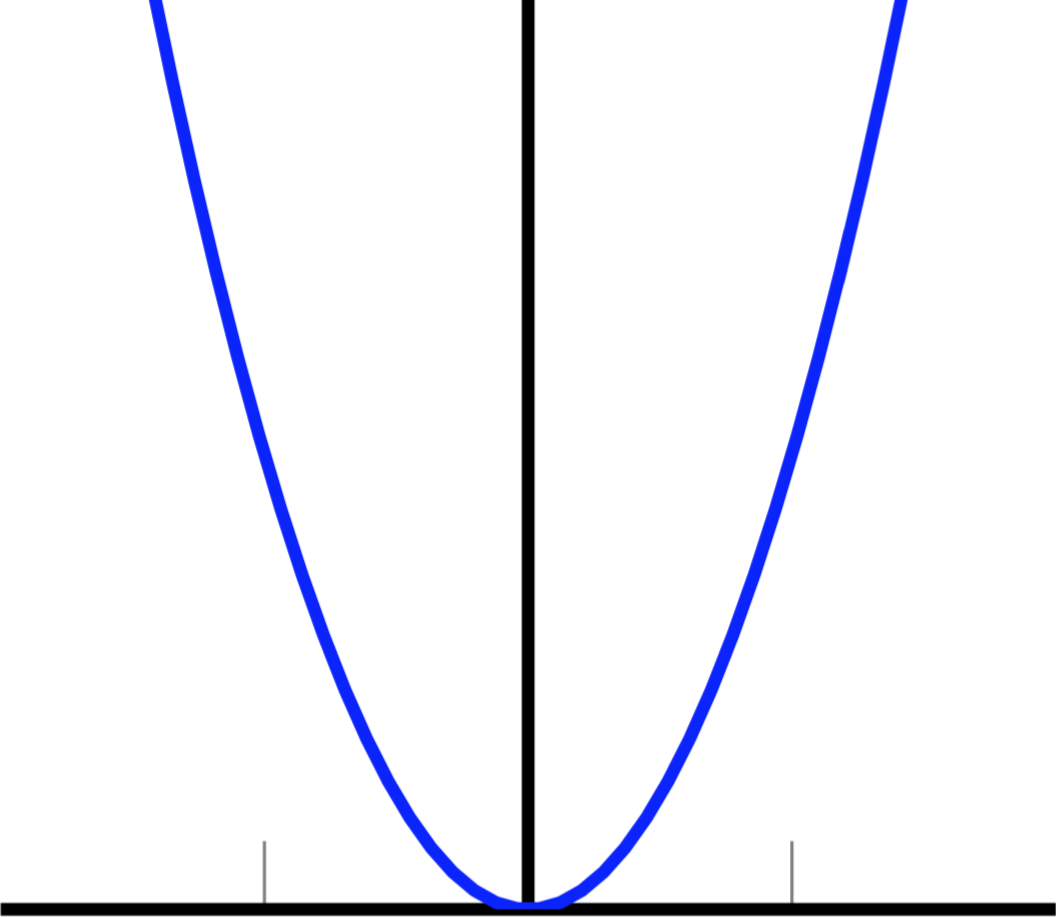
\includegraphics[scale=0.1]{../figures/quadratic} \\
				{\footnotesize Penalizes the outliers quadratically} \\[1ex]
				\hspace{3em} $f(z) = \frac{1}{2}\lVert z\rVert^2$
			\end{block}
		\end{column}
		\begin{column}{0.50\linewidth}
			\begin{block}{Huber Penalty}
				\quad 
				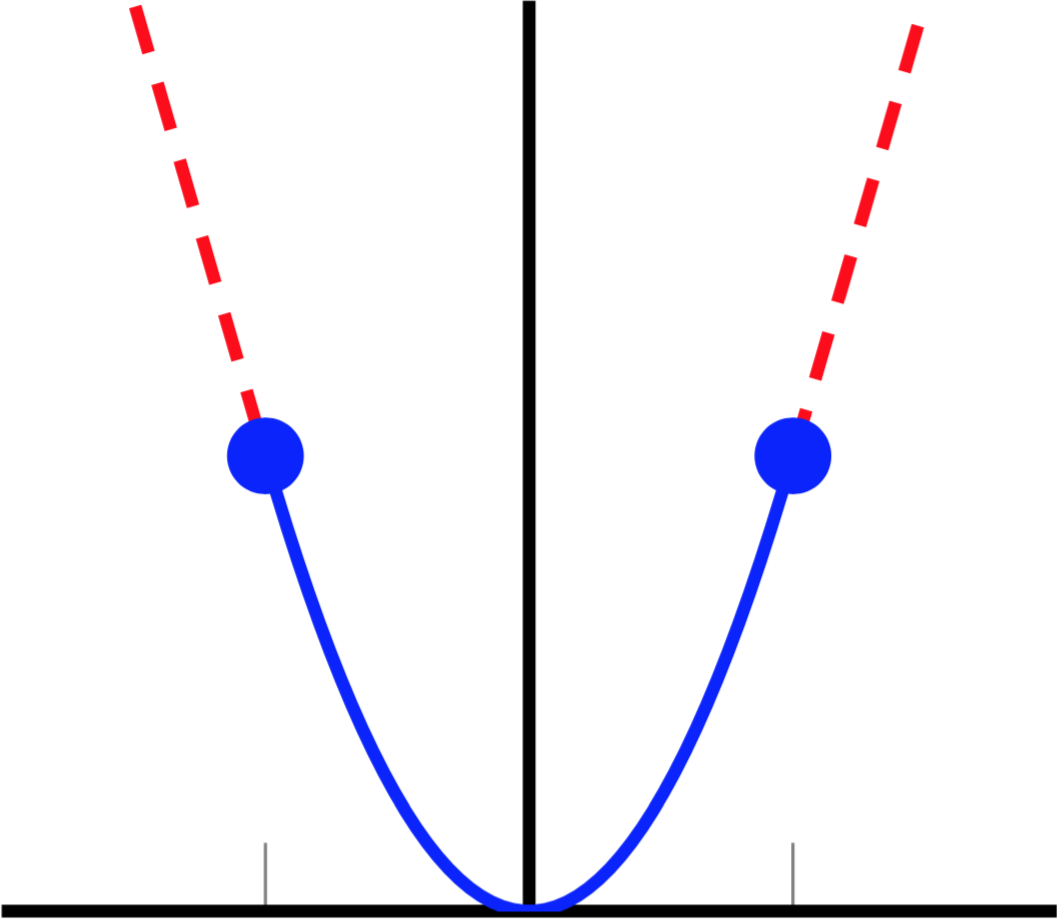
\includegraphics[scale=0.1]{../figures/huber} \\
				{\footnotesize Huber penalty preferred since it is more robust to outliers} \\[1ex]
				$h_{\alpha}(z) = \begin{cases}
				|z|^2& \text{if } |z| \leq \alpha \\
				2\alpha|z| - \alpha^2& \text{if } |z| > \alpha \\
				\end{cases}$
			\end{block}
		\end{column}
	\end{columns}
\end{frame}


\section{Computation}

\begin{frame}
	
	For computational purposes its helpful to rewrite the nested sum with a linear operator,
	
	\[Q = \left( {\begin{array}{*{20}{c}}
		1&{ - 1}&0& \cdots & \cdots &0\\
		1&0&{ - 1}&0& \cdots &0\\
		\vdots & \vdots & \ddots & \ddots & \ddots & \vdots \\
		1&0& \cdots & \cdots &{ - 1}&0\\
		1&0& \cdots & \cdots &0&{ - 1}\\
		0&1&{ - 1}&0& \cdots &0\\
		\vdots & \vdots & \vdots & \vdots & \vdots & \vdots \\
		0& \cdots & \cdots &0&1&{ - 1}
		\end{array}} \right)\]
	
\end{frame}


\begin{frame}{CVX Implementation (Quadratic)}
	\lstinputlisting{../Code/matlab_cvx_norm2.m}
\end{frame}


\begin{frame}{CVX Implementation (Huber)}
	\lstinputlisting{../Code/matlab_cvx_huber.m}
\end{frame}


\begin{frame}
	\begin{center}
		\vspace{-1 mm}
		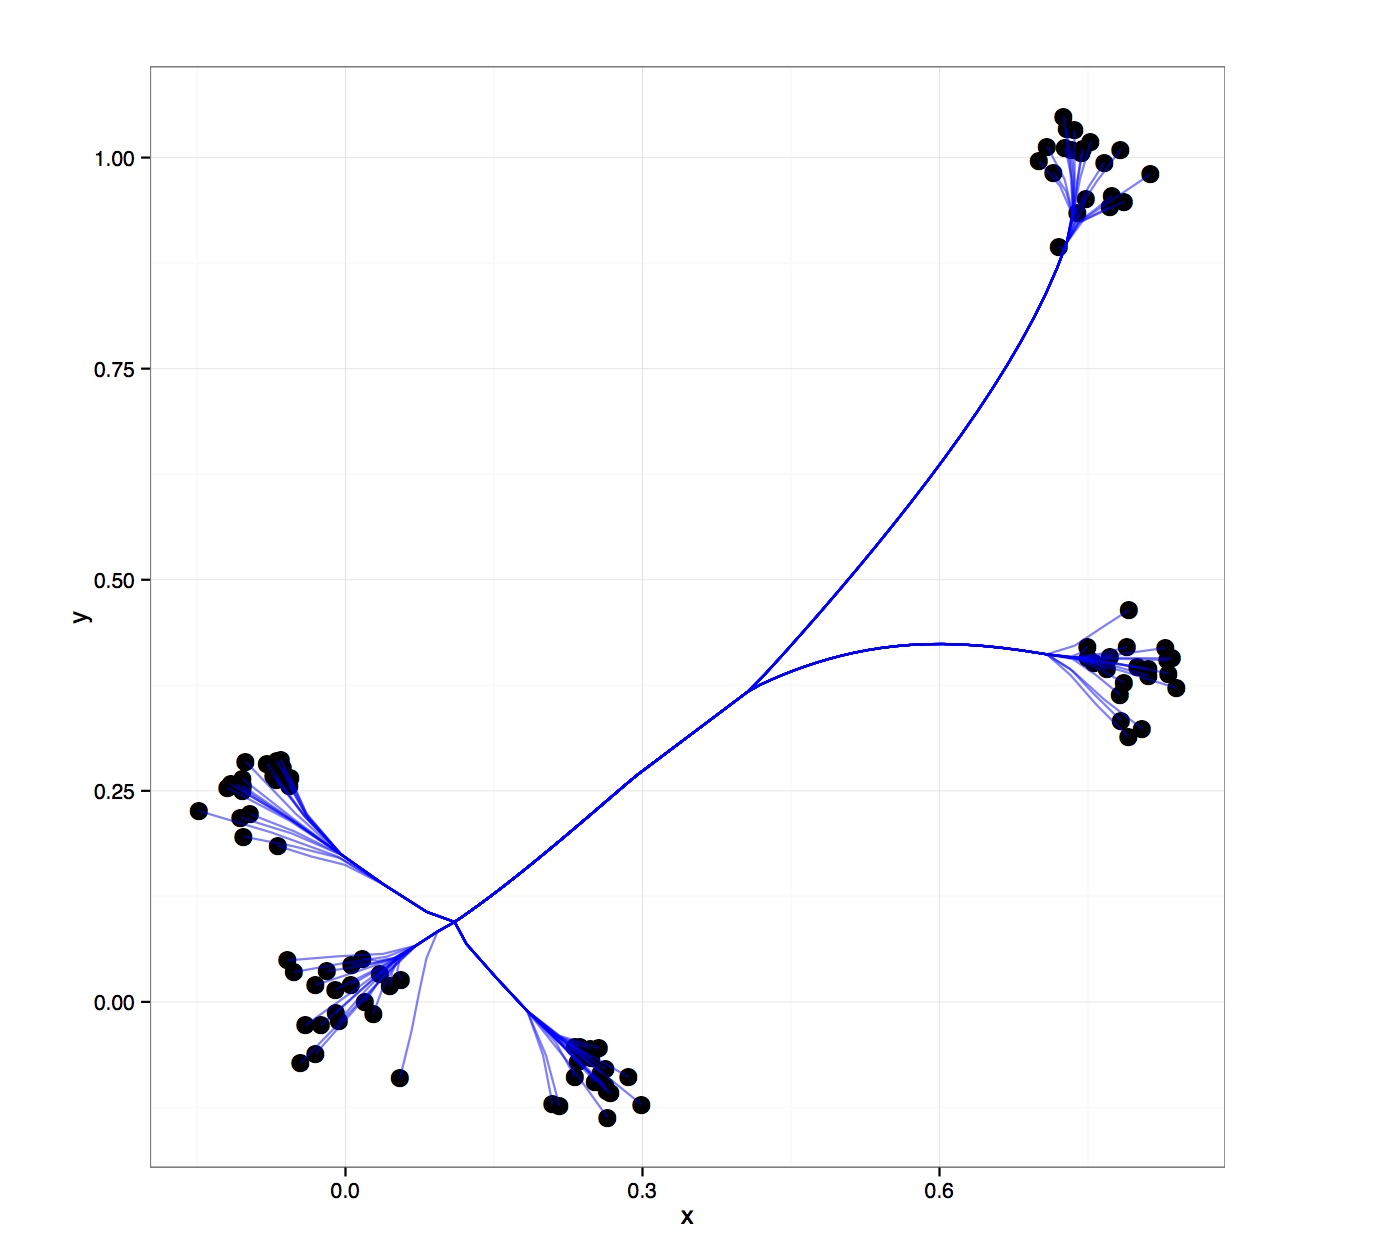
\includegraphics[scale=0.35]{../figures/Clustering_Example.png}
	\end{center}
\end{frame}


\begin{frame}{CVX Implementation (CLS)}
	\lstinputlisting{../Code/matlab_cvx_CLS.m}
\end{frame}



\section{Results}
\begin{frame}
	\begin{center}
		\vspace{-1 mm}
		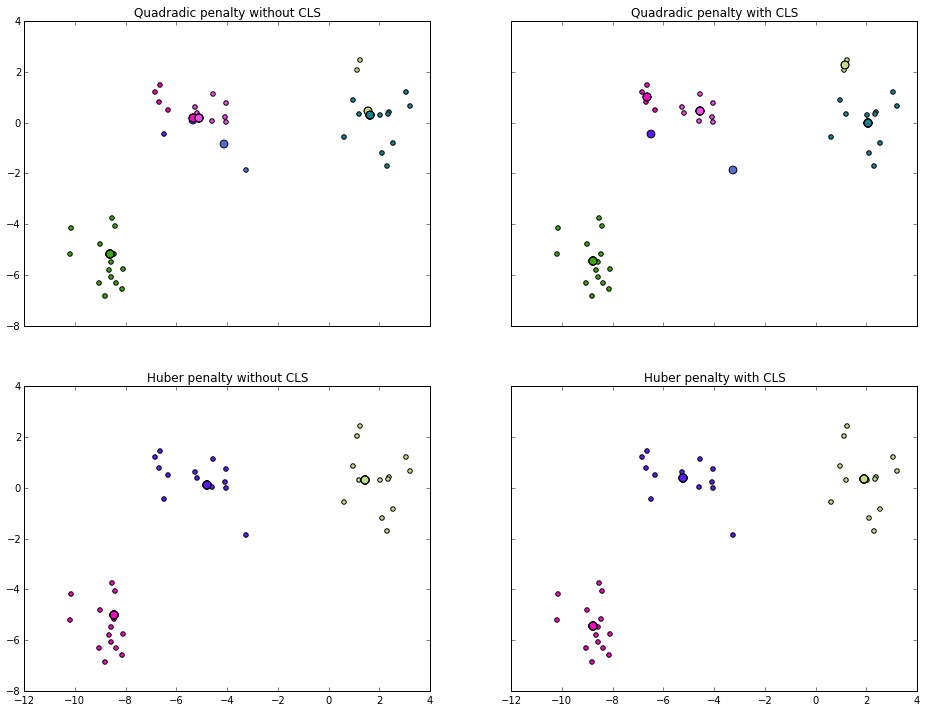
\includegraphics[scale=0.33]{../figures/experiment2.png}
	\end{center}
	
\end{frame}

\section{Discussion}


\begin{frame}{Conclusions}
	
\begin{block}{Kmeans}
	\begin{itemize}
	\item It is fast.\\
	\item Requires the number of clusters as input.
	\item Sensitive to initial conditions.
	\end{itemize}
\end{block}

\begin{block}{Convex Formulation}
\begin{itemize}
\item Only one global minimum.\\
\item Requires a parameter to tune the number of clusters. \\
\item Many ways to exploit structure.
\item Has many other parameters that need tuning.
\end{itemize}
\end{block}




\end{frame}

\begin{frame}{Challenges}
	\begin{itemize}
		\item How can we quantitatively evaluate performance?
		\item How can we optimize parameters without performance metric?
		\item How can we build scalable algorithms?
	\end{itemize}

\end{frame}

\section*{References}
\begin{frame}{\Huge Questions?}
\begin{thebibliography}{10}    
%\setbeamertemplate{bibliography item}[online]
%\bibitem{code} Codes used to generate figures
%\url{https://github.com/snagcliffs/Amath575project}
\beamertemplatebookbibitems % This gives it a nice book symbol


\beamertemplatearticlebibitems % and an article symbol
\bibitem{Wfista} A. Beck and M. Teboulle. A fast iterative shrinkage-thresholding algorithm for linear inverse problem. \textit{SIAM Journal of Imaging Sciences,} 2(1):183-202, 2009.

\bibitem{TVfista}  F. Lindsten and H. Ohlsson. Just Relax and Come Clustering! A Convexification  of k-Means. \textit{Tech. rep., Linko ̈pings universitet 

\end{thebibliography}
\end{frame}

\end{document}
